\documentclass{standalone}
\usepackage{tikz}
\usepackage{ctex,siunitx}
\setCJKmainfont{Noto Serif CJK SC}
\usepackage{tkz-euclide}
\usepackage{amsmath}
\usetikzlibrary{patterns, calc,3d}
\usetikzlibrary {decorations.pathmorphing,decorations.pathreplacing,decorations.shapes,}
\tikzset{label style/.append style={font=\small}}
\begin{document}
\small
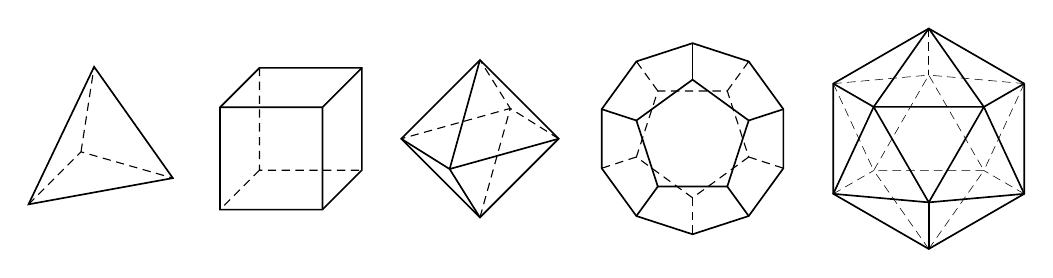
\begin{tikzpicture}[>=latex,scale=1.0]
  \begin{scope}[scale=0.7]
    \foreach \x[count=\i] in {30,90,...,330}
  {
    \tkzDefPoint(\x:2){A\i}
  }
  \foreach \x[count=\i] in {30,150,270}
  {
    \tkzDefPoint(\x:1.1547){B\i}
    \tkzDefPoint(-\x:1.1547){C\i}
  }s
  \tkzDrawPolygon[semithick](A1,A2,A3,A4,A5,A6)
  \tkzDrawPolygon[semithick](B1,B2,B3)
  \tkzDrawPolygon[densely dashed](C1,C2,C3)
  \tkzDrawSegments[semithick](A1,B1 A2,B1 A2,B2 A3,B2 A4,B2 A4,B3 A5,B3 A6,B3 A6,B1)
  \tkzDrawSegments[densely dashed](A1,C1 A2,C3 A3,C2 A3,C3 A4,C2 A5,C2 A5,C1 A6,C1 A1,C3)
  \end{scope}
  \begin{scope}[xshift=-8.5cm,yshift=-0.4cm,scale=1.3]
    \draw[semithick](1,0,0)--(1,1,0)--(0,1,0)--(0,1,1)--(0,0,1)--(1,0,1)--cycle;
    \draw[semithick](0,1,1)--(1,1,1)--(1,1,0)(1,1,1)--(1,0,1);
    \draw[densely dashed](0,1,0)--(0,0,0)--(1,0,0)(0,0,0)--(0,0,1);
  \end{scope}
  \begin{scope}[xshift=-5.7cm]
    \draw[semithick](0,1,0)--(-1,0,0)--(0,-1,0)--(1,0,0)--cycle;
    \draw[semithick](1,0,0)--(0,0,1)--(-1,0,0)(0,-1,0)--(0,0,1)--(0,1,0);
    \draw[densely dashed](1,0,0)--(0,0,-1)--(-1,0,0)(0,-1,0)--(0,0,-1)--(0,1,0);
  \end{scope}
  \begin{scope}[xshift=-10.6cm,yshift=-0.5cm]
    \draw[semithick](-0.5,0,0.866)--(1,0,0)--(0,1.414,0)--cycle;
    \draw[densely dashed](-0.5,0,0.866)--(-0.5,0,-0.866)--(1,0,0)(-0.5,0,-0.866)--(0,1.414,0);
  \end{scope}
  \begin{scope}[xshift=-3.0cm,scale=0.75]
    \foreach \x[count=\i] in {18,90,162,234,306}
    {
      \tkzDefPoint(\x:1){A\i}
      \tkzDefPoint(\x:1.618){AA\i}
      \tkzDefPoint(-\x:1){B\i}
      \tkzDefPoint(-\x:1.618){BB\i}
    }
    \draw[semithick](A1)--(A2)--(A3)--(A4)--(A5)--cycle;
    \draw[densely dashed](B1)--(B2)--(B3)--(B4)--(B5)--cycle;
    \foreach \x in {1,2,3,4,5}
    {
      \draw[semithick](A\x)--(AA\x);
      \draw[densely dashed](B\x)--(BB\x);
    }
    \draw[semithick](AA1)--(BB5)--(AA2)--(BB4)--(AA3)--(BB3)--(AA4)--(BB2)--(AA5)--(BB1)--cycle;
  \end{scope}
\end{tikzpicture}
\end{document}